%GiG
\documentclass{beamer} 
\usetheme{Copenhagen}
\setbeamertemplate{navigation symbols}{}
\setbeamertemplate{headline}{}
\DeclareMathOperator*{\argmax}{arg\,max}

\usepackage{hyperref}


\definecolor{azure}{rgb}{0.0, 0.5, 1.0}
%\newcommand{\tblue}[1]{\textcolor{blue}{#1}}
\newcommand{\tblue}[1]{{\Large {\textcolor{azure}{#1}}}}
\newcommand{\thblue}[1]{{\Huge {\textcolor{azure}{#1}}}}
\newcommand{\hred}[1]{{\textcolor{red}{#1}}}
\newcommand{\furl}[1]{{\footnote{\url{#1}}}}

\newcommand{\mypause}{\pause}
%\newcommand{\mypause}{}

\title[Saravanan Thirumuruganathan] 
{Lecture 3: Principles of Data Visualization}

\author[CSE 5334] 
{Instructor: Saravanan Thirumuruganathan}

\date[] 

\begin{document}

\begin{frame}
  \titlepage
\end{frame}

%\begin{frame}{Outline}
%  \tableofcontents
%  % You might wish to add the option [pausesections]
%\end{frame}

\section{Outline}

\begin{frame}
\frametitle {Outline}
\begin{enumerate}
\item Bertin's Visual Attributes
\item Tufte's Principles
\item Effective Visualization
\item Intro to PsychoPhysics
\end{enumerate}
\end{frame}


\begin{frame}{In-Class Quizzes}
\begin{itemize}
\item {\Large {\bf URL:}} {\LARGE \bf \url{http://m.socrative.com/}} 
\item {\Large {\bf Room Name:} {\LARGE \bf 4f2bb99e}}
\end{itemize}
\end{frame}

\begin{frame}{Announcements} 
    \begin{itemize}
        \item One-time attendance recording
        \item Form teams soon!
        \item Programming Assignment 1 will be released this weekend (due in 3 weeks)
    \end{itemize}
\end{frame}  

\section{Visual Attributes}
\begin{frame}{} 
    \begin{center}
        \thblue{Bertin's Visual Attributes}
    \end{center}
\end{frame}


\section{PsychoPhysics}
\begin{frame}{} 
    \begin{center}
        \thblue{Introduction to PsychoPhysics}
    \end{center}
\end{frame}

\begin{frame}{PsychoPhysics\footnote{From Wikipedia}}
    \begin{itemize}
        \item ``the scientific study of the relation between stimulus and sensation''
        \item ``the analysis of perceptual processes by studying the effect on a subject's experience or behaviour of systematically varying the properties of a stimulus along one or more physical dimensions''
    \end{itemize}
\end{frame}

\begin{frame}{PsychoPhysics\footnote{From Wikipedia}} 
    \begin{itemize}
        \item {\bf Visual Encoding}: the way in which data is mapped into visual structures, upon which we build the images on a screen.
        \item {\bf Visual Perception:} ability to interpret the surrounding environment by processing information that is contained in visible light.
    \end{itemize}
\end{frame}  


\begin{frame}{Effective Visual Encoding} 
    \begin{itemize}
        \item {\bf Challenge:} Pick the best encoding (or mapping) from many possibilities. Consider:
        \begin{itemize}
            \item {\bf Importance Ordering}: Encode the most important information in the most perceptually accurate way
            \item {\bf Expressiveness}: Depict all the data, and only the data
            \item {\bf Consistency}: The properties of the image (visual attributes) should match the properties of the data
        \end{itemize}
    \end{itemize}
\end{frame}  


\begin{frame}{Importance Ordering: Perceptual Properties} 
    \begin{center}
        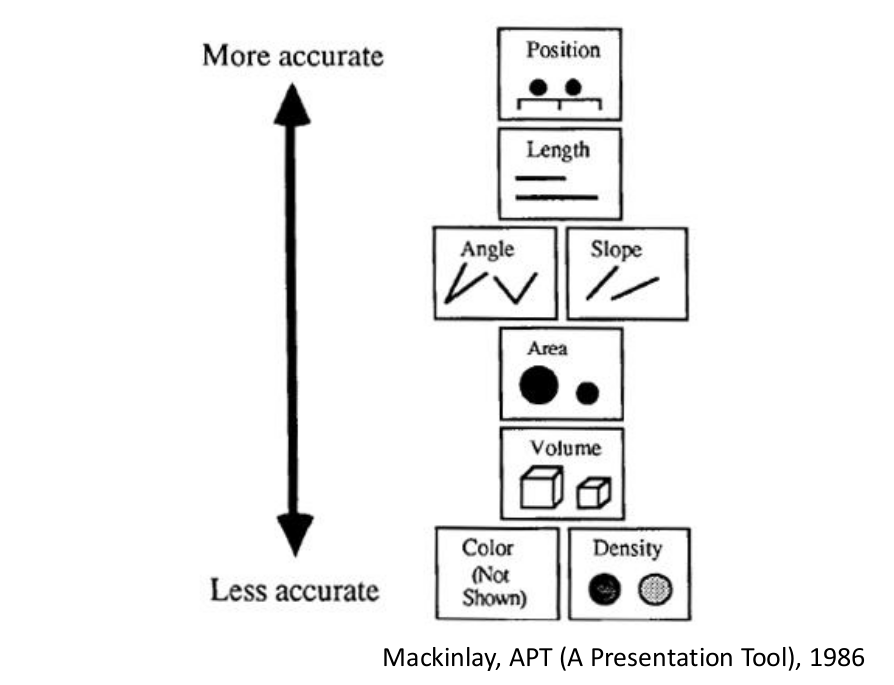
\includegraphics[scale=0.3]{mckinlaysOrdering.png}
    \end{center}
\end{frame}  
\begin{frame}{Expressiveness}
    \begin{center}
        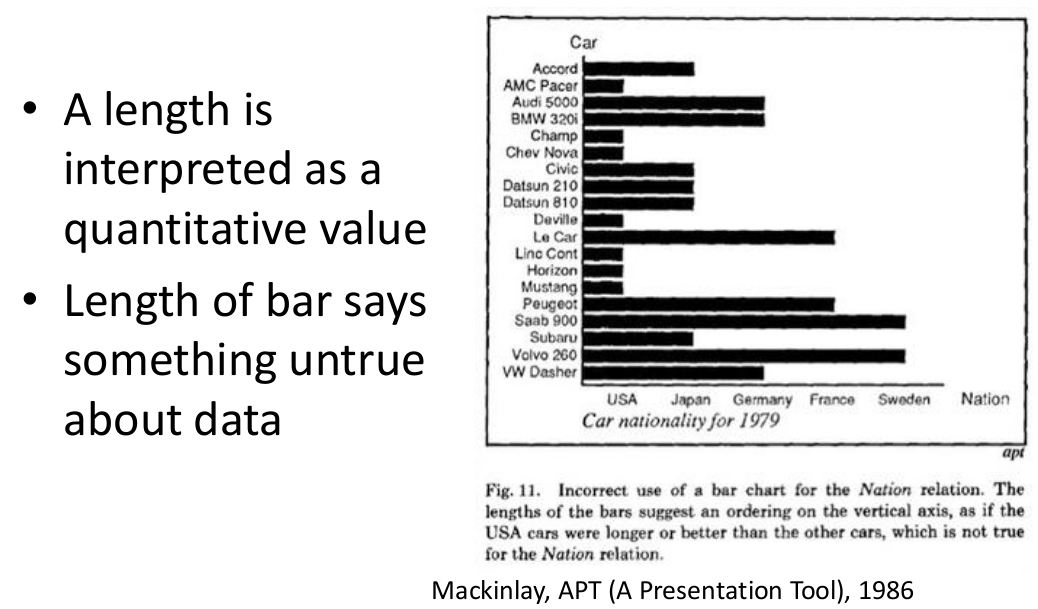
\includegraphics[scale=0.3]{mackinlayExpressiveness.png}
    \end{center}
\end{frame}  
\begin{frame}{Consistency}
    \begin{center}
        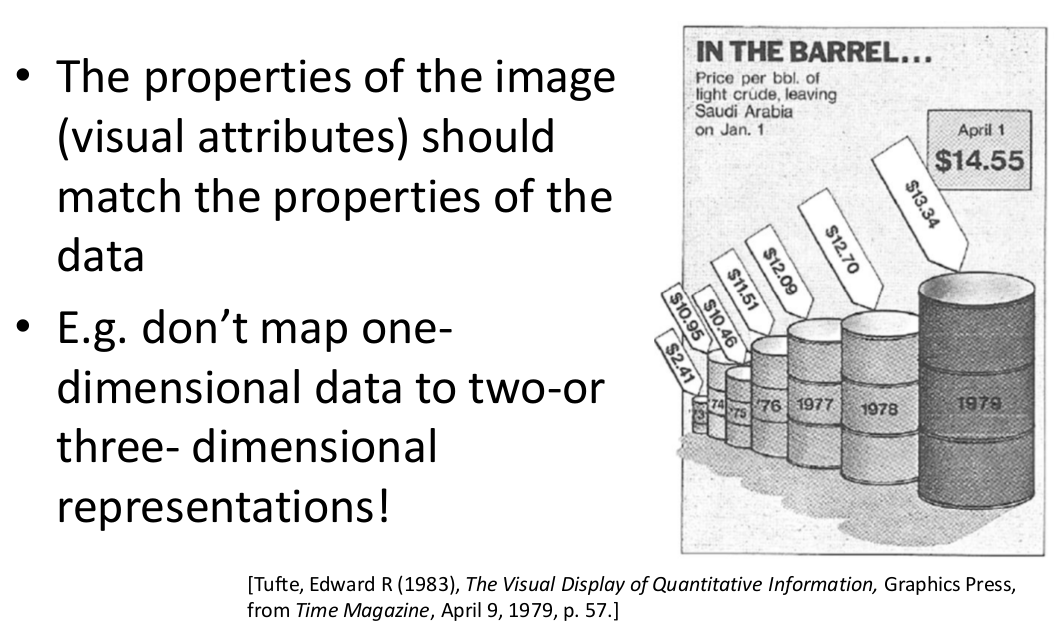
\includegraphics[scale=0.3]{mackinlayConsistency.png}
    \end{center}
\end{frame}  


\begin{frame}{Visual Perception} 
    \begin{itemize}
        \item 70\% of body's sense receptors reside in our eyes
        \item ``The eye and the visual cortex of the brain form a massively parallel processor that provides the highest-bandwidth channel into human cognitive centers.'' Colin Ware, Information Visualization, 2004
        \item Important to understand how visual perception works in order to effectively design visualizations
    \end{itemize}
\end{frame}  


\begin{frame}{How the Eye Works} 
    \begin{itemize}
        \item The eye is not a camera!
        \item Better metaphor for vision: ``dynamic and ongoing construction project'' - Healey, 95
        \item Attention is selective (filtering)
    \end{itemize}
\end{frame}  


\begin{frame}{How to Use Perceptual Properties} 
    \begin{itemize}
        \item Information visualization should cause what is meaningful to stand out
    \end{itemize}
    \begin{center}
        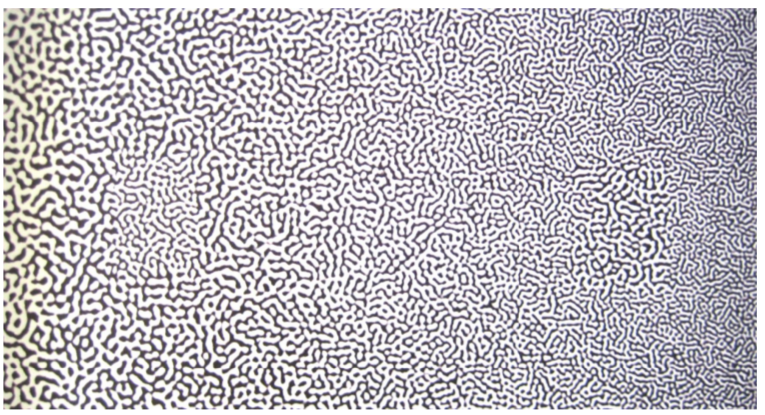
\includegraphics[scale=0.3]{perceptualProperties.png}
    \end{center}
\end{frame}  


\begin{frame}{Eyes vs. Cameras} 
    \begin{itemize}
        \item Cameras
        \begin{itemize}
            \item Good optics
            \item Single focus, white balance, exposure
            \item ``Full image capture''
        \end{itemize}
        \item Eyes
        \begin{itemize}
            \item Relatively poor optics
            \item Constantly scanning (saccades)
            \item Constantly adjusting focus
            \item Constantly adapting (white balance, exposure)
            \item Mental reconstruction of image (sort of)
        \end{itemize}
    \end{itemize}
\end{frame}  

\begin{frame}{}
    \begin{center}
        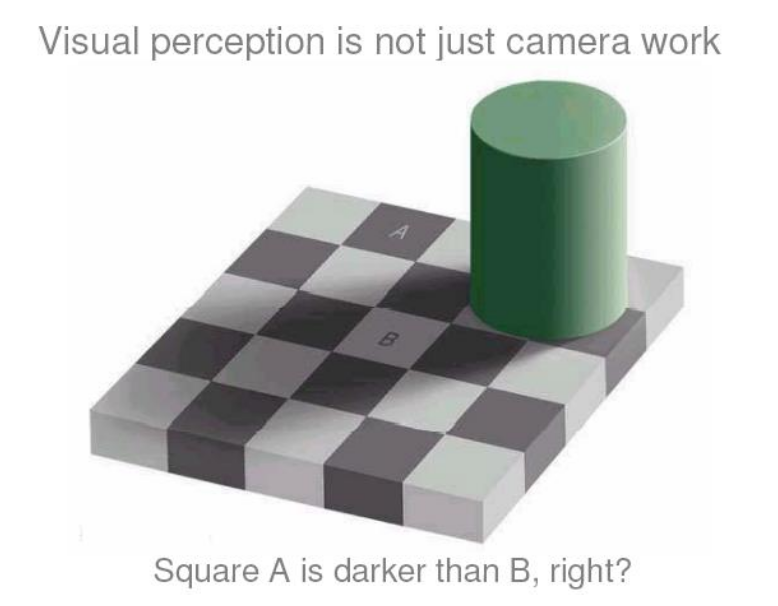
\includegraphics[scale=0.3]{visualParadox1.png}
    \end{center}
\end{frame}  
\begin{frame}{}
    \begin{center}
        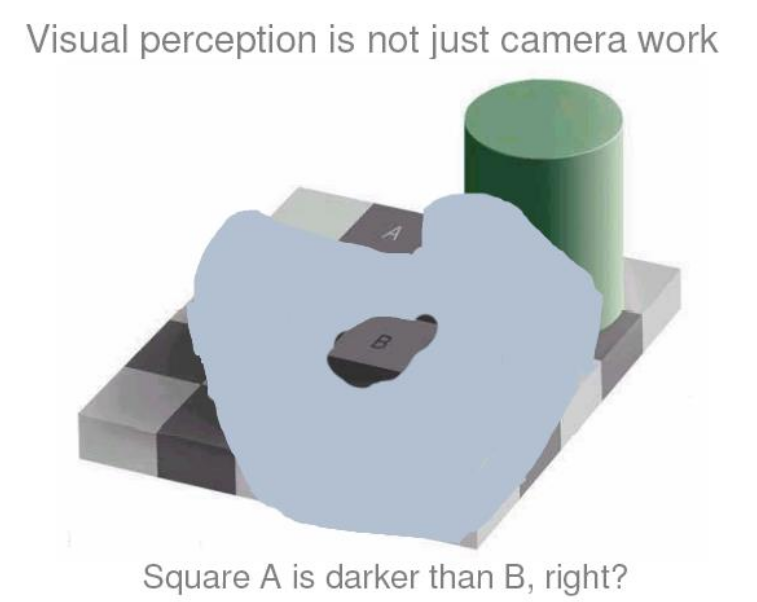
\includegraphics[scale=0.3]{visualParadox2.png}
    \end{center}
\end{frame}  
\begin{frame}{Color is relative}
    \begin{center}
        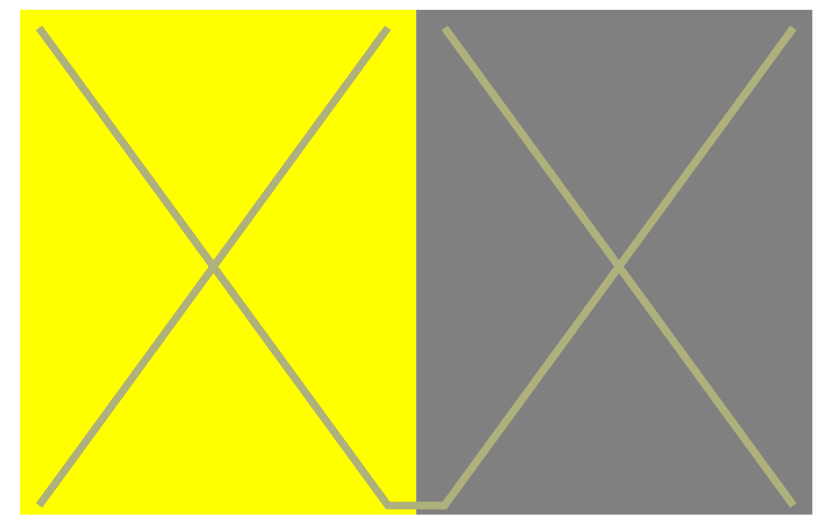
\includegraphics[scale=0.3]{visualParadox3.png}
    \end{center}
\end{frame}  

\begin{frame}{How many 5's} 
    \begin{center}
        385720939823728196837293827 \\
        382912358383492730122894839 \\
        909020102032893759273091428 \\
        938309762965817431869241024 \\
    \end{center}
\end{frame}  
\begin{frame}{How many 5's} 
    \begin{center}
        38\textcolor{red}{5}720939823728196837293827 \\
        3829123\textcolor{red}{5}8383492730122894839 \\
        9090201020328937\textcolor{red}{5}9273091428 \\
        93830976296\textcolor{red}{5}817431869241024 \\
    \end{center}
\end{frame}  

\begin{frame}{Stroop Effect}
    \begin{itemize}
        \item {\bf Stroop Effect:} interference in the reaction time of a task. 
        \begin{enumerate}
            \item \textcolor{green}{Green} \textcolor{red}{Red} \textcolor{blue}{Blue} \\ \textcolor{purple}{Purple} \textcolor{blue}{Blue} \textcolor{purple}{Purple}
            \item \textcolor{red}{Blue} \textcolor{green}{Purple} \textcolor{blue}{Red} \\ \textcolor{blue}{Green} \textcolor{red}{Purple} \textcolor{purple}{Green}
        \end{enumerate}
    \end{itemize}
\end{frame}  


\begin{frame}{Stroop Effect Theories\footnote{From Wikipedia}}
    \begin{enumerate}
        \item brain's ability to recognize the color of the word since the brain reads words faster than it recognizes colors.
        \item color recognition as opposed to reading a word, requires more attention.
        \item recognizing colors is not an ``automatic process'' there is hesitancy to respond; whereas, the brain automatically understands the meaning of words as a result of habitual reading.
        \item brain analyzes information, different and specific pathways are developed for different tasks. Some pathways, such as reading, are stronger than others
    \end{enumerate}
\end{frame}  

\begin{frame}{Semantically Resonant Color Assignments}
    \begin{center}
        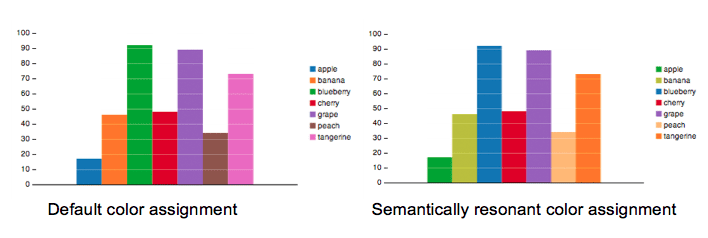
\includegraphics[scale=0.45]{fruitcharts.png}
    \end{center}
\end{frame}

\begin{frame}{Preattentive Processing} 
    \begin{itemize}
        \item Certain basic visual properties are detected immediately by low-level visual system
        \item ``Pop-out'' vs. serial search
        \item $<$ 200 - 250ms qualifies as preattentive 
        \begin{itemize}
            \item eye movements take at least 200ms
            \item yet certain processing can be done very quickly, implying low-level processing in parallel
        \end{itemize}
        \item If a decision takes a fixed amount of time regardless of the number of distractors, it is considered to be {\bf preattentive}.
    \end{itemize}
\end{frame}  


\begin{frame}{Preattentive Processing} 
    \begin{itemize}
        \item A limited set of visual properties are processed preattentively
        \begin{itemize}
            \item (without need for focusing attention).
        \end{itemize}
        \item This is important for design of visualizations
        \begin{itemize}
            \item What can be perceived immediately?
            \item Which properties are good discriminators?
            \item What can mislead viewers?
        \end{itemize}
    \end{itemize}
\end{frame}  

\begin{frame}{Color (Hue) is Preattentive} 
    \begin{itemize}
        \item Detection of red circle in group of blue circles is Preattentive
    \end{itemize}
    \begin{center}
        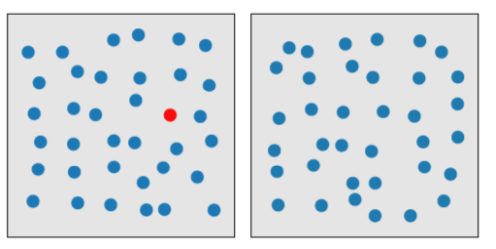
\includegraphics[scale=0.4]{preattentive1.png}
    \end{center}
\end{frame}  

\begin{frame}{Form (curvature) is preattentive} 
    \begin{itemize}
        \item Curved form ``pops out'' of display
    \end{itemize}
    \begin{center}
        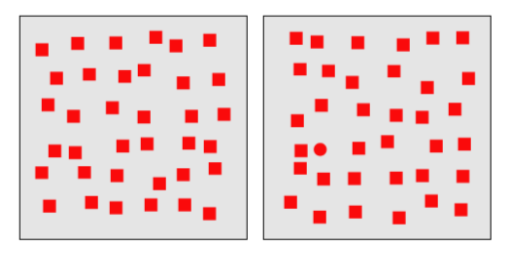
\includegraphics[scale=0.4]{preattentive2.png}
    \end{center}
\end{frame}  

\begin{frame}{Conjunction of Attributes} 
    \begin{itemize}
        \item Conjunction target generally cannot be detected preattentively (red circle in sea of red square and blue circle distractors)
    \end{itemize}
    \begin{center}
        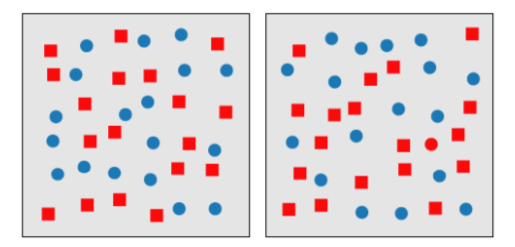
\includegraphics[scale=0.4]{preattentive3.png}
    \end{center}
\end{frame}  

\begin{frame}{Separability of Attributes}
    \begin{center}
        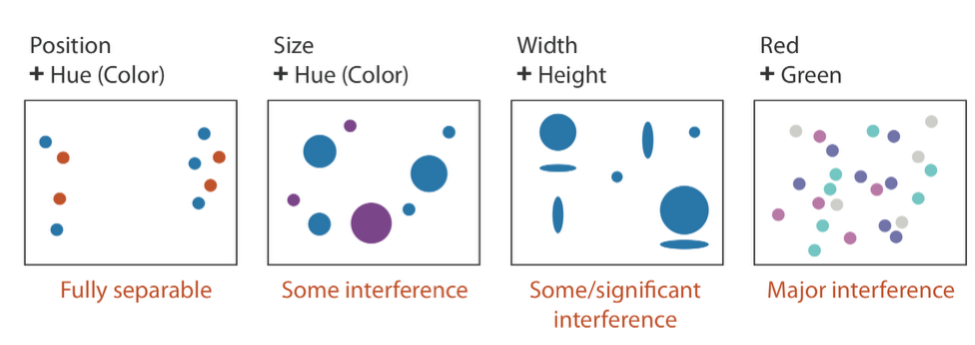
\includegraphics[scale=0.3]{separabilityOfAttributes.png}
    \end{center}
\end{frame}  
\begin{frame}{Visual Popout (Preattentive Features) - I}
    \begin{center}
        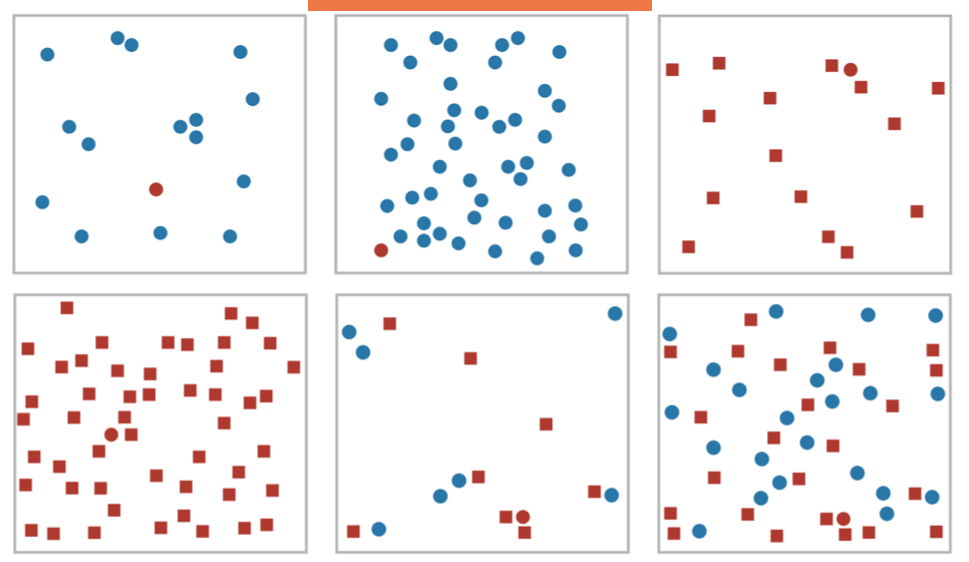
\includegraphics[scale=0.3]{preAttentiveFeatures.png}
    \end{center}
\end{frame}  
\begin{frame}{Visual Popout (Preattentive Features) - II}
    \begin{center}
        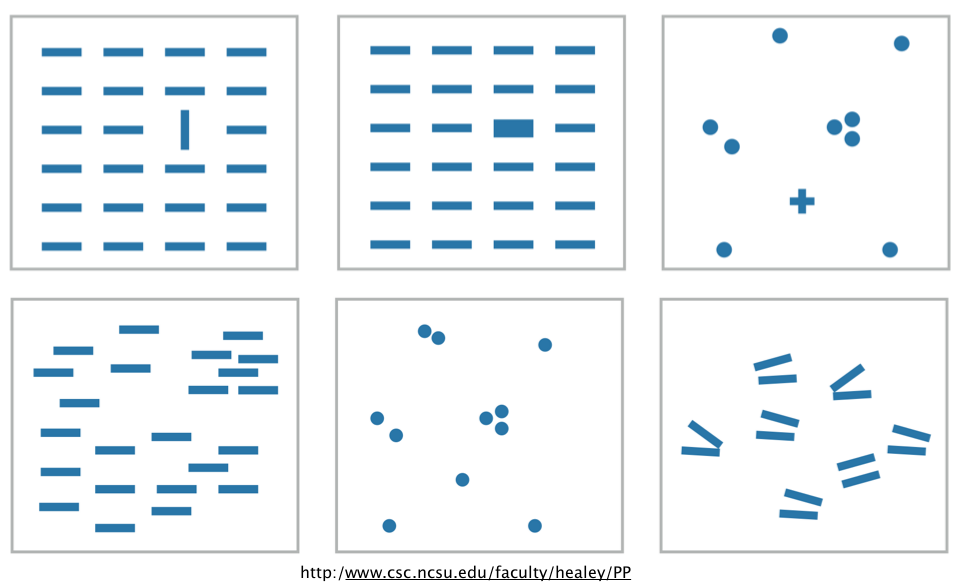
\includegraphics[scale=0.3]{preAttentiveFeatures2.png}
    \end{center}
\end{frame}  
\begin{frame}{Feature Hierarchy}
    \begin{center}
        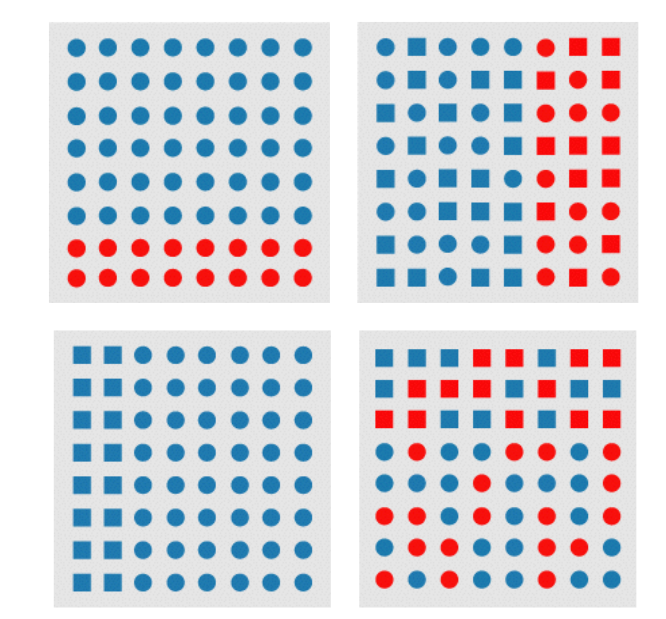
\includegraphics[scale=0.3]{featureHierarchy.png}
    \end{center}
\end{frame}  
\begin{frame}{Grouping Principles}
    \begin{center}
        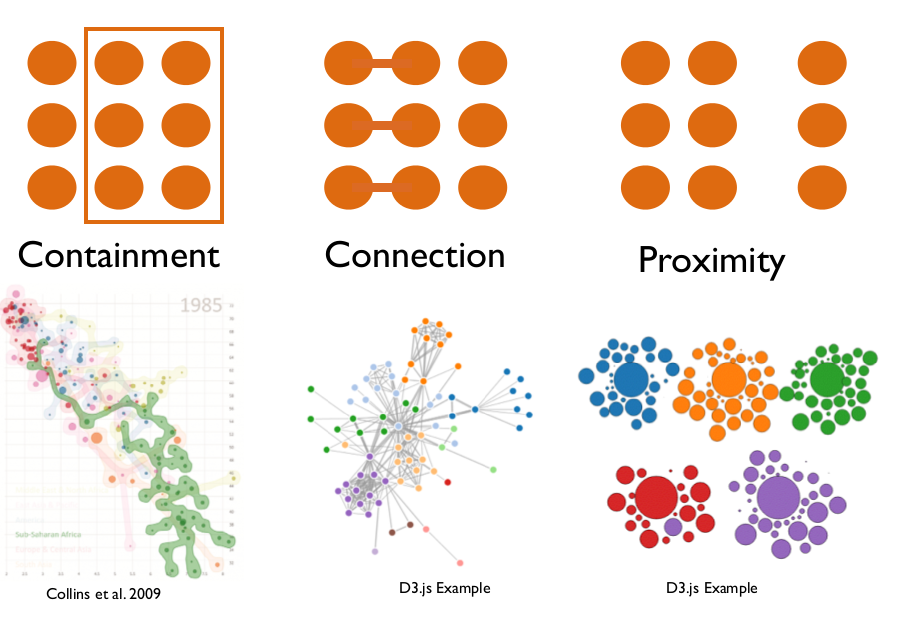
\includegraphics[scale=0.3]{groupingPrinciples.png}
    \end{center}
\end{frame}  
\begin{frame}{Grouping Principles}
    \begin{center}
        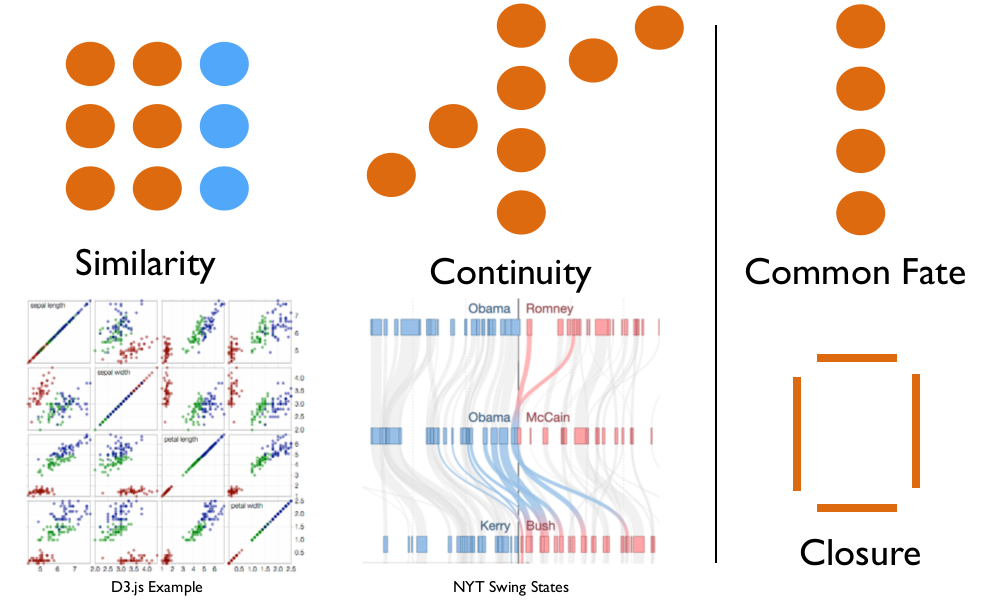
\includegraphics[scale=0.3]{groupingPrinciples2.png}
    \end{center}
\end{frame}  
\begin{frame}{Munzner Hierarchy}
    \begin{center}
        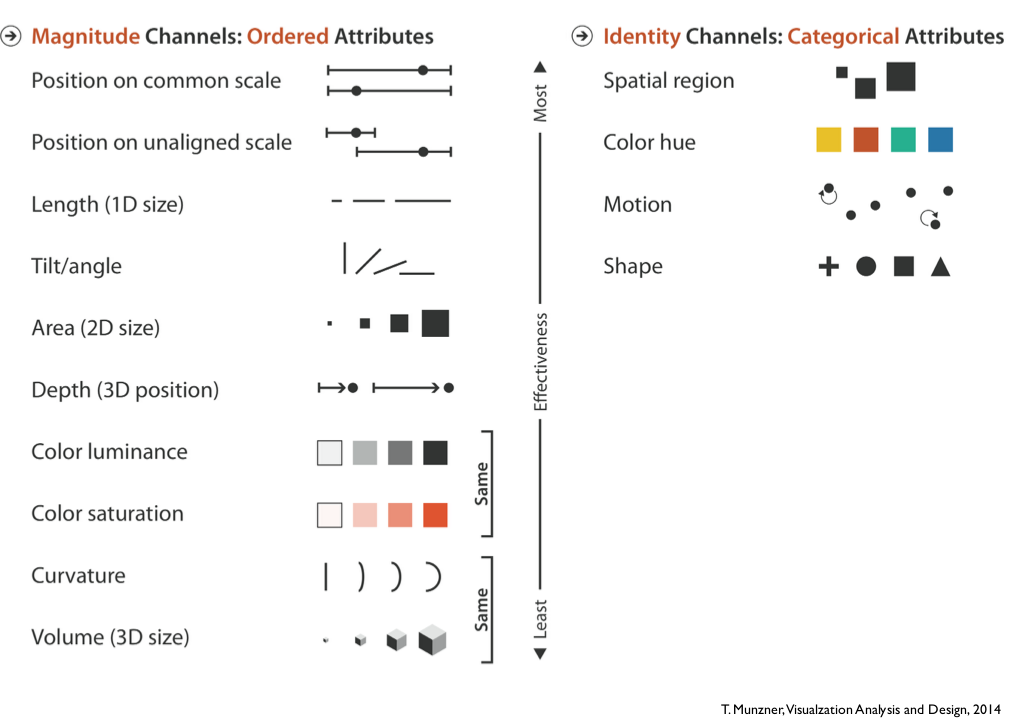
\includegraphics[scale=0.3]{munznerHierarchy.png}
    \end{center}
\end{frame}  

\begin{frame}{Preattentive Visual Properties (Healey 97)}
    \begin{center}
        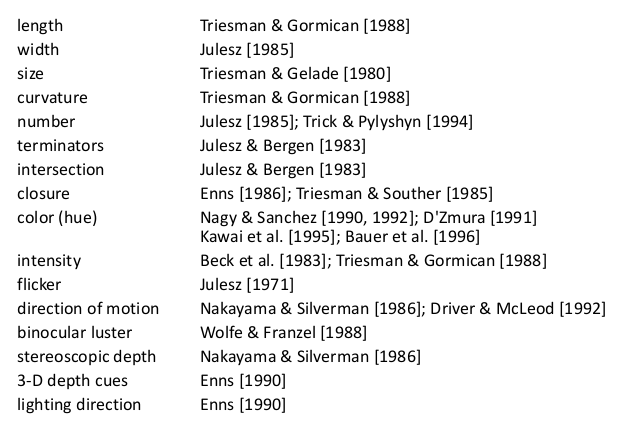
\includegraphics[scale=0.3]{preattentiveVisProperties.png}
    \end{center}
\end{frame}  

\begin{frame}{Critiquing a Visualization} 
    \begin{enumerate}
        \item First, consider the purpose of the visualization and who the intended audience is.
        \item Then, ascertain your initial reaction.
        \item Then, examine the visualization in detail.
        \item Then, answer questions like the following.
    \end{enumerate}
\end{frame}  

\begin{frame}{Over-Arching Questions} 
    \begin{enumerate}
        \item Is the design visually appealing/aesthetically pleasing?
        \item Is it immediately understandable? If not, is it understandable after a short period of study?
        \item Does it provide insight or understanding that was not obtainable with the original representation (text, table, etc)?
        \item Does it provide insight or understanding better than some alternative visualization would? Or does it require excessive cognitive effort? What kind of visualization might have been better?
    \end{enumerate}
\end{frame}  

\begin{frame}{How Successful is the Visualization?} 
    \begin{enumerate}
        \setcounter{enumi}{4}
        \item Does the visualization reveal trends, patterns, gaps, and/or outliers? Can the viewer make effective comparisons?
        \item Does the visualization successfully highlight important information, while providing context for that information?
        \item Does it distort the information? If it transforms it in some way, is this misleading or helpfully simplifying?
        \item Does it omit important information?
        \item Is it memorable?
    \end{enumerate}
\end{frame}  

\begin{frame}{Questions about the Visual Transformation} 
    \begin{enumerate}
        \setcounter{enumi}{9}
        \item Does it use visual components properly?
        \begin{itemize}
            \item Does it properly represent the data using lines, color, position, etc?
            \item Does it transform nominal, ordinal, and quantitative information properly?
        \end{itemize}
        \item Does it use labels and legends appropriately?
    \end{enumerate}
\end{frame}  



\section{Summary}

\begin{frame}{Summary}

\tblue{Major Concepts:}
\begin{itemize}
    \item Visual Attributes
    \item Principles of effective visualization
    \item Visual encoding and perception
\end{itemize}
\end{frame}

\begin{frame}{Slide Material References}

\begin{itemize}
    \item Slides from Harvard CS 109 (2013 and 2014)
    \item Slides by Cecilia Aragon
\end{itemize}
\end{frame}


\end{document}

